\documentclass{beamer}


\usepackage[no-math]{fontspec}
\usepackage{xunicode}
\usepackage{xltxtra}
\usepackage{bm}
\usepackage{tikz}
\usepackage{graphicx}
\usepackage{relalg}
\usepackage{booktabs}
\usepackage{hyperref}


% Beamer setup
\usefonttheme{structurebold}
\useinnertheme{rectangles}
\usenavigationsymbolstemplate{}
\setbeamertemplate{footline}[frame number]


% TikZ setup
\usetikzlibrary{positioning}
\usetikzlibrary{graphs}
\usetikzlibrary{decorations.pathreplacing}
\usetikzlibrary{calc}
\usetikzlibrary{arrows}


% fontspec setup
\defaultfontfeatures{Mapping=tex-text}
\setsansfont[Scale=MatchUppercase,BoldFont={Gill Sans}]{Gill Sans Light}
\setmonofont[Scale=MatchLowercase]{Letter Gothic 12 Pitch}


% graphicx setup
\graphicspath{{images/}}


% custom macros
% "empty" arrow tip
\pgfarrowsdeclare{:}{:}{}{}
% custom bar arrow tip, offset from end of line (use "empty" tip at line ends if no >)
\tikzset{crossbar/.tip={|[scale width=1.75,sep=0.25em]}}
% various edge styles for TikZ
\tikzset{
    function/.style={arrows={->}},
    injection/.style={arrows={<-}},
    total/.style={arrows={:{crossbar}-}},
    surjection/.style={arrows={-{crossbar}:}},
    bijection/.style={arrows={<{crossbar}-{crossbar}>}},
    projection/.style={arrows={:{crossbar}-{crossbar}>}},
    projection left/.style={arrows={:{crossbar}-{crossbar}>},edge label={\scriptsize\(\RelProject\)}},
    projection right/.style={arrows={:{crossbar}-{crossbar}>},edge label'={\scriptsize\(\RelProject\)}},
    selection left/.style={arrows={<-{crossbar}>},edge label={\scriptsize\(\RelRestrict\)}},
    selection right/.style={arrows={<-{crossbar}>},edge label'={\scriptsize\(\RelRestrict\)}},
    funcdep left/.style={arrows={->},edge node={node[sloped,midway,above] {\scriptsize\emph{key}}}},
    funcdep right/.style={arrows={->},edge node={node[sloped,midway,below] {\scriptsize\emph{key}}}},
    surtotal/.style={arrows={:{crossbar}-{crossbar}:}},
    input keep/.style={structure,thick},
    input delete/.style={structure!40,thick,dashed},
    output/.style={alert,thick},
    output temp/.style={alert,thick,dashed},
    path 1/.style={green!60!black,thick},
    path 2/.style={orange,thick},
    invisible/.style={opacity=0},
    visible on/.style={alt=#1{}{invisible}},
    input on/.style={alt=#1{input keep}{}},
    output on/.style={alt=#1{output}{}},
    alt/.code args={<#1>#2#3}{\alt<#1>{\pgfkeysalso{#2}}{\pgfkeysalso{#3}}}
}
        
% projection and selection edge annotations for TikZ
\newcommand{\ProjectionAnnotation}[3][]{%
    \path (#2) to node[above,#1] {\scriptsize\(\RelProject\)} (#3);%
}
\newcommand{\SelectionAnnotation}[3][]{%
    \path (#2) to node[above,#1] {\scriptsize\(\RelRestrict\)} (#3);%
}


\newcounter{constraint}

% misc
\newcommand{\todo}[1]{\textbf{!!TODO!!} {[#1]}}

% commonly used elements
\newcommand{\LS}{\ensuremath{\mathit{LS}}}
\newcommand{\NLS}{\ensuremath{\mathit{NLS}}}
\newcommand{\LSsub}{\ensuremath{\mathit{L}}}
\newcommand{\NLSsub}{\ensuremath{\mathit{N}}}
\newcommand{\Sno}{\ensuremath{\mathit{Sno}}}
\newcommand{\Sname}{\ensuremath{\mathit{Sname}}}
\newcommand{\Status}{\ensuremath{\mathit{Status}}}
\newcommand{\City}{\ensuremath{\mathit{City}}}

\newcommand{\Type}[1]{\ensuremath{T_{#1}}}
\newcommand{\TT}[1]{\ensuremath{T_{\{#1\}}}}

\newcommand{\CityLondon}{\ensuremath{\{\City\colon\allowbreak\text{`\emph{London}'}\}}}
\newcommand{\TCityMinusLondon}{\ensuremath{\Type{\City} \setminus \CityLondon}}
\newcommand{\TSSC}{\ensuremath{\Type{\Sname} \times \Type{\Status} \times \Type{\City}}}
\newcommand{\TSSL}{\ensuremath{\Type{\Sname} \times \Type{\Status} \times \CityLondon}}
\newcommand{\TSSNL}{\ensuremath{\Type{\Sname} \times \Type{\Status} \times (\TCityMinusLondon)}}

\newcommand{\TLSPlusNLS}{\ensuremath{\Type{\LS} + \Type{\NLS}}}
\newcommand{\TTLSPlusNLS}{\ensuremath{\TT{\LS} + \TT{\NLS}}}
\newcommand{\TLSPlusNLSsub}{\ensuremath{\Type{\LSsub} + \Type{\NLSsub}}}
\newcommand{\TTLSPlusNLSsub}{\ensuremath{\TT{\LSsub} + \TT{\NLSsub}}}

\newcommand{\StackTLSPlusNLS}{\ensuremath{\begin{array}{c}\Type{\LS}\,+ \\ \Type{\NLS}\end{array}}}
\newcommand{\StackTTLSPlusNLS}{\ensuremath{\begin{array}{c}\TT{\LS}\,+ \\ \TT{\NLS}\end{array}}}
\newcommand{\StackTLSPlusNLSsub}{\ensuremath{\begin{array}{c}\Type{\LSsub}\,+ \\ \Type{\NLSsub}\end{array}}}
\newcommand{\StackTTLSPlusNLSsub}{\ensuremath{\begin{array}{c}\TT{\LSsub}\,+ \\ \TT{\NLSsub}\end{array}}}
\newcommand{\StackTSSC}{\ensuremath{\begin{array}{c}\Type{\Sname}\,\times \\ \Type{\Status} \times \Type{\City}\end{array}}}
\newcommand{\StackTSSL}{\ensuremath{\begin{array}{c}\Type{\Sname} \times \Type{\Status}\,\times \\ \CityLondon\end{array}}}
\newcommand{\StackTSSNL}{\ensuremath{\begin{array}{c}\Type{\Sname} \times \Type{\Status}\,\times \\ (\TCityMinusLondon)\end{array}}}
\newcommand{\StackTCityMinusLondon}{\ensuremath{\begin{array}{c}\Type{\City}\,\setminus \\ \CityLondon\end{array}}}

\newcommand{\SC}[1]{\ensuremath{\mathcal{S}_{#1}}}

% dominates
\newcommand{\Dominates}[2]{\ensuremath{#2 \preceq #1}}
\newcommand{\Equivalent}[2]{\ensuremath{#1 \equiv #2}}

% SIG notation (in text)
\newcommand{\Sedge}[1]{\ensuremath{\sigma_{\textrm{#1}}}}
\newcommand{\SedgeP}[1]{\ensuremath{\sigma_{\textrm{#1}}^{'}}}

\newcommand{\medmid}{\raise.125ex\hbox{\scalebox{1}[0.75]{$\mid$}}}

% General SIG edges for use in formulas.
% Adapted from: http://tex.stackexchange.com/questions/96330/adding-symbols-at-the-ends-of-a-horizontal-line
\makeatletter
\newlength{\@annotskipleft}
\newlength{\@annotskipright}
% #1 = left edge component
% #2 = right edge component
% #3 = left bar annotation
% #4 = right bar annotation
\newcommand\@sig@edge[4]{%
    \let\@middle\joinrel%
    \ifx#1\relbar%
        \@annotskipleft=.3em%
        % scrunch up the bare line so it's similar length to \long...arrow
        \ifx#2\relbar\def\@middle{\joinrel\joinrel\relbar\joinrel\joinrel}\fi%
    \else% 
        % arrows need a little more clearance
        \@annotskipleft=.4em%
    \fi%
    \ifx#2\relbar\@annotskipright=.3em\else\@annotskipright=.4em\fi%
    \mathrel{\ooalign{$#1\@middle#2$\cr\hskip\@annotskipleft$#3$\hfil$#4$\hskip\@annotskipright\cr}}%
}

% 0 = nothing
% 1 = bar
% 2 = arrowhead
% 3 = both
\def\@sigedge#1#2{%
    \ifcase\numexpr#1*4+#2\relax%
        \@sig@edge{\relbar}{\relbar}{}{}\or                     % 00 = -----
        \@sig@edge{\relbar}{\relbar}{}{\medmid}\or              % 01 = ---+-
        \@sig@edge{\relbar}{\rightarrow}{}{}\or                 % 02 = ---->
        \@sig@edge{\relbar}{\rightarrow}{}{\medmid}\or          % 03 = ---+>
        \@sig@edge{\relbar}{\relbar}{\medmid}{}\or              % 10 = -+---
        \@sig@edge{\relbar}{\relbar}{\medmid}{\medmid}\or       % 11 = -+-+-
        \@sig@edge{\relbar}{\rightarrow}{\medmid}{}\or          % 12 = -+-->
        \@sig@edge{\relbar}{\rightarrow}{\medmid}{\medmid}\or   % 13 = -+-+>
        \@sig@edge{\leftarrow}{\relbar}{}{}\or                  % 20 = <----
        \@sig@edge{\leftarrow}{\relbar}{}{\medmid}\or           % 21 = <--+-
        \@sig@edge{\leftarrow}{\rightarrow}{}{}\or              % 22 = <--->
        \@sig@edge{\leftarrow}{\rightarrow}{}{\medmid}\or       % 23 = <--+>
        \@sig@edge{\leftarrow}{\relbar}{\medmid}{}\or           % 30 = <+---
        \@sig@edge{\leftarrow}{\relbar}{\medmid}{\medmid}\or    % 31 = <+-+-
        \@sig@edge{\leftarrow}{\rightarrow}{\medmid}{}\or       % 32 = <+-->
        \@sig@edge{\leftarrow}{\rightarrow}{\medmid}{\medmid}   % 33 = <+-+>
    \fi%
}

\newcommand{\sigedge}[1]{\ensuremath{\@sigedge#1}}
\makeatother

\newcommand{\Edge}{\sigedge{00}}
\newcommand{\Total}{\sigedge{10}}
\newcommand{\Surjective}{\sigedge{01}}
\newcommand{\SurTotal}{\sigedge{11}}
\newcommand{\Functional}{\sigedge{02}}
\newcommand{\Injective}{\sigedge{20}}
\newcommand{\Bijective}{\sigedge{33}}

% Hack to get the overset symbols to appear at the right height.
% \smash removes the spacing around the operator, hence \mathop.
\newcommand{\LabelledEdge}[2]{\mathop{\overset{\raisebox{0.3em}{\scriptsize\ensuremath{#2}}}{\smash[t]{#1}}}}
\newcommand{\ProjectionEdge}{\LabelledEdge{\sigedge{13}}{\RelProject}}
\newcommand{\SelectionEdge}{\LabelledEdge{\sigedge{23}}{\RelRestrict}}
\newcommand{\TrivialProjection}{\ensuremath{\LabelledEdge{\Bijective}{\RelProject}}}
\newcommand{\TrivialSelection}{\ensuremath{\LabelledEdge{\Bijective}{\RelRestrict}}}
\newcommand{\KeyEdge}{\ensuremath{\LabelledEdge{\Functional}{\mathit{key}}}}

% Constraints.
\newcommand{\Constraint}[2][]{C\ensuremath{_{#2}\ifx&#1&\else^{#1}\fi}}
\newenvironment{ConstraintList}[1][]{%
    \begin{list}{%
        \bfseries%
        \ifx&#1&%
            \Constraint{\ensuremath{\bm{\arabic{constraint}}}}%
        \else%
            \Constraint[\ensuremath{\bm{#1}}]{\ensuremath{\bm{\arabic{constraint}}}}%
        \fi%
    }%
    {\usecounter{constraint}}%
}{\end{list}}


% Draw a grid to aid TikZ picture drawing/debugging.
\newcommand{\DrawGridTikZ}[2]{%
	\begin{scope}[color=lightgray]
		\draw[thin,step=1mm]  (0.0,0.0)   grid (#1,#2);%
		\draw[thick,step=1cm] (-0.1,-0.1) grid (#1+0.1,#2+0.1);%
		\pgftext[top,at={\pgfxy(0.0,-0.2)}]{\tiny 0}%
		\pgftext[right,at={\pgfxy(-0.2,0.0)}]{\tiny 0}%
		\foreach \x in {1,...,#1} {\pgftext[top,at={\pgfxy(\x,-0.2)}]{\tiny\x}}%
		\foreach \y in {1,...,#2} {\pgftext[right,at={\pgfxy(-0.2,\y)}]{\tiny\y}}%
	\end{scope}
}


% Sometimes we want to put a comment in tiny text on the next line, but the default line skip
% will insert too much vertical space. Put a \tinyskip at the end of the line instead.
\def\tinyskip{\\[-0.33\baselineskip]}


% Bold-face text using the structure colour.
\newcommand<>{\structurebf}[1]{\structure#2{\textbf{#1}}}


% preamble
\title{Characterising relational view updates \\ using relative information capacity}
\author{Nigel Stanger \\ \footnotesize Information Science}
\date{August 19, 2016}


\begin{document}


%%%%%%%%%%%%%%%%%%%%%%%%%%%%%%%%%%%%%%%%%%%%%%%%%%%%%%%%%%%%%%%%%%%%%%%%%%%%%%%%


\frame
{
    \thispagestyle{empty}
    \titlepage
}


%%%%%%%%%%%%%%%%%%%%%%%%%%%%%%%%%%%%%%%%%%%%%%%%%%%%%%%%%%%%%%%%%%%%%%%%%%%%%%%%


\section{The Problem}


%%%%%%%%%%%%%%%%%%%%%%%%%%%%%%%%%%%%%%%%%%%%%%%%%%%%%%%%%%%%%%%%%%%%%%%%%%%%%%%%


\frame{\tableofcontents}


%%%%%%%%%%%%%%%%%%%%%%%%%%%%%%%%%%%%%%%%%%%%%%%%%%%%%%%%%%%%%%%%%%%%%%%%%%%%%%%%


\frame
{
    \centering
    \begin{tikzpicture}
        \node (book) {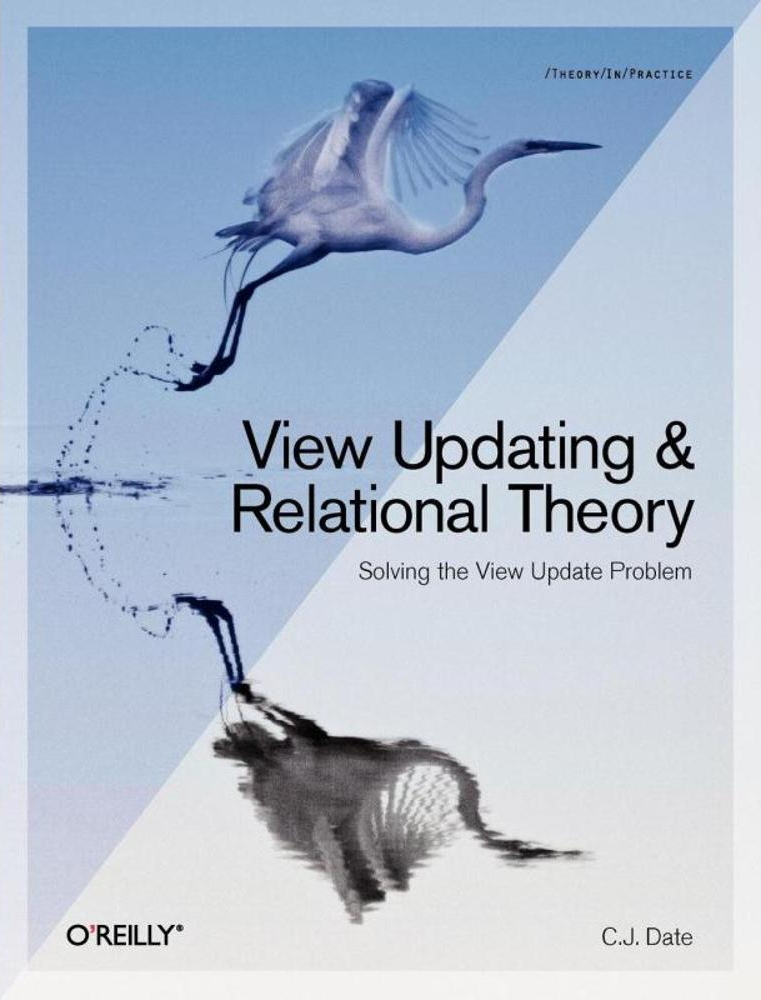
\includegraphics[height=8cm,keepaspectratio]{Date-ViewUpdatingandRelationalTheory-large.png}};
        \node[anchor=north] (url) at (book.south) {\tiny\href{http://shop.oreilly.com/product/0636920028437.do}{http://shop.oreilly.com/product/0636920028437.do} (2013)};
        \node (date) [below=0.8cm of book.east] {
\includegraphics[height=2.2cm,keepaspectratio]{date.png}};
        \only<2->{\fill[fill,yellow,semitransparent] (-0.25,-0.75) rectangle (2.55,-0.4);}
%         \DrawGridTikZ{7.0}{8.0}
    \end{tikzpicture}
}


%%%%%%%%%%%%%%%%%%%%%%%%%%%%%%%%%%%%%%%%%%%%%%%%%%%%%%%%%%%%%%%%%%%%%%%%%%%%%%%%


\frame
{
    \frametitle{Some quick terminology}
    
    \begin{columns}
        \begin{column}{0.4\textwidth}
            \centering
            
\includegraphics[width=0.95\columnwidth,keepaspectratio]{Date-SQLandRelationalTheory.png}
            
            \tiny\href{http://shop.oreilly.com/product/0636920022879.do}{http://shop.oreilly.com/product/0636920022879.do} \\
            (second edition, 2011)
            
            \note<1>[item]{This is the second edition; the third edition is now available.}
        \end{column}
        \begin{column}{0.6\textwidth}
            \structurebf{Value vs.\ variable}
            \begin{itemize}
                \item a value is immutable (“2”)
                \item a variable contains a value
                \item[\(\Rightarrow\)] \emph{relation} value, variable (\emph{relvar})
            \end{itemize}
            \medskip
            
            \structurebf{Relation \alert<2>{heading} \& \alert<3>{body}}
            \medskip
            
            {\scriptsize
            \begin{tabular}{c|l|l|r|l|}
                \cline{2-5}
                \textbf{S}  &   \textbf{\alert<2>{Sno}} &   \textbf{\alert<2>{Sname}}   &   \textbf{\alert<2>{Status}}  &   \textbf{\alert<2>{City}}    \\
                \cline{2-5}
                            &   \alert<3>{S1}           &   \alert<3>{Smith}            &   \alert<3>{20}               &   \alert<3>{London}   \\
                            &   \alert<3>{S2}           &   \alert<3>{Jones}            &   \alert<3>{30}               &   \alert<3>{Paris}    \\
                \cline{2-5}
            \end{tabular}}
            \bigskip
            
            \structurebf{Type (\(\bm{\Type{x}}\))}
            \begin{itemize}
                \item (finite) set of values that something can take
            \end{itemize}
            \medskip
            
            \structurebf{Date doesn’t believe in nulls}\tinyskip
            {\tiny (but it doesn’t really matter here)}
        \end{column}
    \end{columns}
}


%%%%%%%%%%%%%%%%%%%%%%%%%%%%%%%%%%%%%%%%%%%%%%%%%%%%%%%%%%%%%%%%%%%%%%%%%%%%%%%%


\frame
{
    \frametitle{Some quick terminology}
    
    \structurebf{Attribute type (\(\bm{\Type{A}}\))}
    \begin{itemize}
        \item set of all possible values that \(A\) can take
        \item[=] \(\{v_{1}, v_{2}, \dotsc, v_{m}\}\) {\tiny (for finite \(m\))}
    \end{itemize}
    \medskip
    
    \structurebf{Tuple type (\(\bm{\TT{R}}\)) of relvar \(\bm{R}\)}
    \begin{itemize}
        \item set of all possible tuple values with \(R\)’s heading
        \item[=] Cartesian product of \(R\)’s attribute types
        \item[=] \(\Type{A_{1}} \times \Type{A_{2}} \times \dotsb \times \Type{A_{n}}\)
    \end{itemize}
    \medskip
    
    \structurebf{Relation type (\(\bm{\Type{R}}\)) of relvar \(\bm{R}\)}
    \begin{itemize}
        \item set of all possible relation values with \(R\)’s heading
        \item[=] every possible combination of elements of \(\TT{R}\)
    \end{itemize}
}


%%%%%%%%%%%%%%%%%%%%%%%%%%%%%%%%%%%%%%%%%%%%%%%%%%%%%%%%%%%%%%%%%%%%%%%%%%%%%%%%


\frame
{
    \frametitle{Date’s (hoary and clichéd) suppliers-and-parts schema}
    
    \structurebf{\(\bm{S\{\Sno, \Sname, \Status, \City\}}\)}
    
    \begin{quote}
        \upshape
        Supplier \(\Sno\) is under contract, is named \(\Sname\), has status \(\Status\), and is located in city \(\City\)
    \end{quote}
    \bigskip
    
    \structurebf{\(\bm{P\{\mathit{Pno}, \mathit{Pname}, \mathit{Colour}, \mathit{Weight}, \City\}}\)}
    
    \begin{quote}
        \upshape
        Part \(\mathit{Pno}\) is used in the enterprise, is named \(\mathit{Pname}\), has colour \(\mathit{Colour}\), and weight \(\mathit{Weight}\)
    \end{quote}
    \bigskip
    
    \structurebf{\(\bm{SP\{\Sno, \mathit{Pno}, \mathit{Qty}\}}\)}
    
    \begin{quote}
        \upshape
        Supplier \(\Sno\) supplies part \(\mathit{Pno}\) in quantity \(\mathit{Qty}\)
    \end{quote}
}


%%%%%%%%%%%%%%%%%%%%%%%%%%%%%%%%%%%%%%%%%%%%%%%%%%%%%%%%%%%%%%%%%%%%%%%%%%%%%%%%


\frame
{
    \frametitle{The view update problem}

    \centering
    \Large
    \begin{tikzpicture}[every edge/.style={draw,semithick}]
        \node (vdb)                         {\(V(\mathit{DB})\)};
        \node (db)   [below=18mm of vdb]    {\(\mathit{DB}\vphantom{(')}\)};

        \node (vdbp) [right=4cm of vdb]     {\(V(\mathit{DB}')\)};
        \node (uvdb) [left=-1mm of vdbp]    {\(U(V(\mathit{DB})) \stackrel{?}{=}\)};

        \node (dbp)  at (db -| vdbp)        {\(\mathit{DB}\smash[t]{'}\vphantom{()}\)};
        \node (tudb) [left=-1mm of dbp]     {\(T(U)(\mathit{DB}) =\)};

        \graph{
            { (db), (dbp) } -> [edge label={\(V\)},swap] { (vdb), (vdbp) };

            (vdb) -> [edge node={node (u)  [above=-0.6mm] {\(U\)}}]    (uvdb);
            (db)  -> [edge node={node (tu) [above=-0.6mm] {\(T(U)\)}}] (tudb);

            (u)   -> [double equal sign distance=2pt,-implies,edge label={\(T\)}] (tu);
        };
    \end{tikzpicture}
    \\
    \tiny Keller (1985) \emph{Algorithms for translating view updates to database updates for views involving selections, projections, and joins}
    
    \note<1>{Keller: “The user specifies update \(U\) against the view of the database, \(V(\mathit{DB})\). The view update translator \(T\) supplies the database update \(T(U)\), which results in \(DB'\) when applied to the database. The new view state is \(V(\mathit{DB}')\). This translation has no side effects in the view if \(V(\mathit{DB}') = U(V(\mathit{DB}))\), that is, if the view has changed precisely in accordance with the user’s request.”}
    
    \bigskip
    \normalsize
    
    \begin{uncoverenv}<2->
        \structurebf{Problem:} there are often multiple update translations \(T(U)\) that produce the effect of \(U\) but have quite different effects on \(\mathit{DB}\).
        \bigskip
    
        How do we choose?
    \end{uncoverenv}
}


%%%%%%%%%%%%%%%%%%%%%%%%%%%%%%%%%%%%%%%%%%%%%%%%%%%%%%%%%%%%%%%%%%%%%%%%%%%%%%%%


\frame
{
    \frametitle{The view update problem}
    
    \begin{columns}
        \begin{column}[T]{0.45\textwidth}
            \footnotesize\color{gray!70}
            \begin{tabular}{|l|l|r|l|}
                \multicolumn{4}{l}{\textbf{S}}  \\
                \hline
                \textbf{Sno}        &   \textbf{Sname}      &   \textbf{Status}     &   \textbf{City}   \\
                \hline
                S1                  & Smith                 & 20                    & London \\
                S2                  & Jones                 & 30                    & Paris \\
                S3                  & Blake                 & 30                    & Paris \\
                \only<1-2,4->{S4}  & \only<1-2,4->{Clark} & \only<1-2,4->{20}    & \only<1-2,4,6>{London}\only<5>{\alert{???}}\only<7->{\alert{Paris}} \\
                S5                  & Adams                 & 30                    & Athens \\
                \hline
            \end{tabular}
        \end{column}
        \begin{column}[T]{0.45\textwidth}
            \footnotesize
            \begin{tabular}{|l|l|r|l|}
                \multicolumn{4}{l}{\(\bm{\text{\textbf{LS}} = \RelRestrict_{\text{\textbf{City}} = \text{\textbf{`London'}}} \,\text{\textbf{S}}}\)}  \\
                \hline
                \textbf{Sno}    &   \textbf{Sname}  &   \textbf{Status} &   \textbf{City}   \\
                \hline
                S1              & Smith             & 20                & London \\
                \only<1-2,4,6>{S4} & \only<1-2,4,6>{Clark}& \only<1-2,4,6>{20}   & \only<1-2,4,6>{London} \\
                \hline
            \end{tabular}
        \end{column}
    \end{columns}
    \bigskip
    
    \structurebf{Delete S4 from LS?}
    
    \begin{enumerate}
        \item<2-> Delete S4 from S.
        \item<4-> Change S4’s city to anything other than London.
    \end{enumerate}
    \bigskip
    
    \begin{uncoverenv}<6->
        \structurebf{What if we instead \emph{change} S4’s city to Paris in LS?}
        \begin{itemize}
            \item<7->[\(\Rightarrow\)] changing S4’s city to Paris in S
            \item<7-> side effect: some changes behave like deletes!
        \end{itemize}
    \end{uncoverenv}
}


%%%%%%%%%%%%%%%%%%%%%%%%%%%%%%%%%%%%%%%%%%%%%%%%%%%%%%%%%%%%%%%%%%%%%%%%%%%%%%%%


\frame
{
    \frametitle{The view update problem}
    
%     \structurebf{What about \(\bm{\mathsf{SSP} = \mathsf{S} \RelNaturalJoin \mathsf{SP}}\)?}
    
    \tiny
    \begin{columns}
        \begin{column}[T]{0.35\textwidth}
            \color{gray!70}
            \begin{tabular}{|l|l|r|l|}
                \multicolumn{4}{l}{\textbf{S}}  \\
                \hline
                \textbf{Sno}        &   \textbf{Sname}      &   \textbf{Status}     &   \textbf{City}   \\
                \hline
                \only<1-6,8>{S1}\only<7>{\alert{S6}} & \only<1-8>{Smith} & \only<1-8>{20} & \only<1-8>{London} \\
                S2                  & Jones                 & 30                    & Paris \\
                S3                  & Blake                 & 30                    & Paris \\
                S4                  & Clark                 & 20                    & London \\
                S5                  & Adams                 & 30                    & Athens \\
                \hline
            \end{tabular}
            \bigskip
            
            \begin{tabular}{|l|l|r|}
                \multicolumn{3}{l}{\textbf{SP}}  \\
                \hline
                \textbf{Sno}        &   \textbf{Pno}      &   \textbf{Qty}   \\
                \hline
                \only<1-2,4,6,8>{S1}\only<5>{\alert{S3}}\only<7>{\alert{S6}} & \only<1-2,4-8>{P1} & \only<1-2,4-8>{300} \\
                S1 & P2 & 200 \\
                S1 & P3 & 400 \\
                S1 & P4 & 200 \\
                S1 & P5 & 100 \\
                S1 & P6 & 100 \\
                S2 & P1 & 300 \\
                S2 & P2 & 400 \\
                S3 & P2 & 200 \\
                S4 & P2 & 300 \\
                S4 & P4 & 300 \\
                S4 & P5 & 400 \\
                \hline
            \end{tabular}
        \end{column}
        \begin{column}[T]{0.55\textwidth}
            \begin{tabular}{|l|l|r|l|l|r|}
                \multicolumn{4}{l}{\(\bm{\mathsf{SSP} = \mathsf{S} \RelNaturalJoin \mathsf{SP}}\)}  \\
                \hline
                \textbf{Sno}        &   \textbf{Sname}      &   \textbf{Status}     &   \textbf{City}   &   \textbf{Pno}    &   \textbf{Qty}   \\
                \hline
                \only<1-2,4,6,8>{S1}\only<5>{\alert{S3}}\only<7>{\alert{S6}} & \only<1-2,4,6-8>{Smith}\only<5>{\alert{Blake}} & \only<1-2,4,6-8>{20}\only<5>{\alert{30}} & \only<1-2,4,6-8>{London}\only<5>{\alert{Paris}} & \only<1-2,4-8>{P1} & \only<1-2,4-8>{300} \\
                \only<1-6,8>{S1}\only<7>{\alert{S6}} & \only<1-8>{Smith} & \only<1-8>{20} & \only<1-8>{London} & \only<1-8>{P2} & \only<1-8>{200} \\
                \only<1-6,8>{S1}\only<7>{\alert{S6}} & \only<1-8>{Smith} & \only<1-8>{20} & \only<1-8>{London} & \only<1-8>{P3} & \only<1-8>{400} \\
                \only<1-6,8>{S1}\only<7>{\alert{S6}} & \only<1-8>{Smith} & \only<1-8>{20} & \only<1-8>{London} & \only<1-8>{P4} & \only<1-8>{200} \\
                \only<1-6,8>{S1}\only<7>{\alert{S6}} & \only<1-8>{Smith} & \only<1-8>{20} & \only<1-8>{London} & \only<1-8>{P5} & \only<1-8>{100} \\
                \only<1-6,8>{S1}\only<7>{\alert{S6}} & \only<1-8>{Smith} & \only<1-8>{20} & \only<1-8>{London} & \only<1-8>{P6} & \only<1-8>{100} \\
                S2 & Jones & 30 & Paris & P1 & 300 \\
                S2 & Jones & 30 & Paris & P2 & 400 \\
                S3 & Blake & 30 & Paris & P2 & 200 \\
                S4 & Clark & 20 & London & P4 & 300 \\
                S4 & Clark & 20 & London & P5 & 400 \\
                S4 & Clark & 20 & London & P2 & 200 \\
                \hline
            \end{tabular}
            \bigskip
            
            \scriptsize
            \structurebf{Delete first row of SSP?}
            
            \begin{enumerate}
                \item<2-> Delete \(\mathsf{SP}\{\mathsf{S1}, \mathsf{P1}, \mathsf{300}\}\).
                \item<4-> Change supplier number in \(\mathsf{SP}\{\mathsf{S1}, \mathsf{P1}, \mathsf{300}\}\).
                \item<6-> Change S1’s supplier number in S.
                \item<8-> Delete S1 from S. {\tiny (nuclear option)}
            \end{enumerate}
            \smallskip
            
            \uncover<10>{\structurebf{Changes are even more problematic}}
        \end{column}
    \end{columns}
}


%%%%%%%%%%%%%%%%%%%%%%%%%%%%%%%%%%%%%%%%%%%%%%%%%%%%%%%%%%%%%%%%%%%%%%%%%%%%%%%%


\frame
{
    \frametitle{Date's solution}
    
    \begin{itemize}
    
        \item \emph{All} constraints explcitly specified in advance.
        
        \item Automatically generate \emph{compensatory rules} from constraints.\tinyskip
        {\tiny (kind of like declarative triggers)}
        
        \item No problem if original and view schemas are \emph{information equivalent} (no hidden information).
        \begin{itemize}
        
            \item[] ``if and only if the constraints that apply to [schema \(\SC{1}\)] and [schema \(\SC{2}\)] are such that every proposition that can be represented by [\(\SC{1}\)] can be represented by [\(\SC{2}\)] and vice versa''
        
        \end{itemize}
        \bigskip
        
        \item[BUT:] Still potential for ambiguity when views hide information.
        \bigskip
                
        \item Date’s approach involves “\emph{…a clear element of pragma…}”.\tinyskip
        {\tiny (essentially argues for the “most sensible” ambiguity resolution)}
    
    \end{itemize}
}


%%%%%%%%%%%%%%%%%%%%%%%%%%%%%%%%%%%%%%%%%%%%%%%%%%%%%%%%%%%%%%%%%%%%%%%%%%%%%%%%


\frame
{
    \frametitle{Relative information capacity}
    \framesubtitle{}
    
    \begin{itemize}
    
        \item “Information content” of a schema. {\tiny (including constraints)}
        
        \item Determines set of all valid instances of a schema.
        
        \item Can only be compared, not quantitatively measured.
        \begin{description}
            \item[equivalence] \(\Equivalent{\SC{1}}{\SC{2}}\)
            \item[dominance] \(\Dominates{\SC{2}}{\SC{1}}\)
        \end{description}
        
        \item Mappings between schemas can preserve:
        \begin{description}
            \item[information] information capacity increases (\(\Rightarrow\Dominates{\SC{2}}{\SC{1}}\))
            \item[equivalence] information capacity stays the same (\(\Rightarrow\Equivalent{\SC{1}}{\SC{2}}\))
        \end{description}
    
    \end{itemize}
    
    \flushright\tiny
    Hull (1986) \emph{Relative information capacity of simple relational database schemata} \\
    Miller (1993) \emph{The use of information capacity in schema integration and translation}
}


%%%%%%%%%%%%%%%%%%%%%%%%%%%%%%%%%%%%%%%%%%%%%%%%%%%%%%%%%%%%%%%%%%%%%%%%%%%%%%%%


\frame
{
    \frametitle{Schema intension graphs (SIGs)}
    
    \structurebf{Nodes = typed domains (sets of values)}
    \begin{itemize}
        \item simple
        \item constructed (\(\times\), \(+\))
    \end{itemize}
    \medskip
    
    \structurebf{Edges = associations between domains} {\tiny (binary relations)}
    \begin{itemize}
        \item Simple constraints:
        \begin{itemize}
            \item total (\(A \Total B\)): defined for all \(a \in A\)
            \item surjective (\(A \Surjective B\)): defined for all \(b \in B\)
            \item functional (\(A \Functional B\)): \(a\) maps to at most one \(b\)
            \item injective (\(A \Injective B\)): \(b\) maps to at most one \(a\)
            \item bijective (\(A \Bijective B\)): all four
        \end{itemize}
        \item Selection (\(A \SelectionEdge B\)): \(B\) is a subset of \(A\). {\tiny (specialisation)}
        \item Projection (\(A \ProjectionEdge B\)): \(B\) is a projection of \(A\). {\tiny (\(\Rightarrow A\) is constructed)}
    \end{itemize}

    \flushright\tiny
    Miller (1993) \emph{Schema intension graphs: A formal model for the study of schema equivalence}
}


%%%%%%%%%%%%%%%%%%%%%%%%%%%%%%%%%%%%%%%%%%%%%%%%%%%%%%%%%%%%%%%%%%%%%%%%%%%%%%%%


\frame
{
    \frametitle{Example SIG for relvar S}
    
    \centering\Large
    \begin{tikzpicture}[level distance=18mm]
        \node (TS) {\(\Type{S}\)};
        \node (TTS) [right=1.5cm of TS] {\(\TT{S}\)}
            [sibling distance=4.5cm]
            child[arrows={:{crossbar}-{crossbar}>}] {node (TSno) {\(\Type{\Sno}\)}}
            child[arrows={:{crossbar}-{crossbar}>}] {node (TSSC) {\(\TSSC\)}
                [sibling distance=22mm]
                child[arrows={:{crossbar}-{crossbar}>}] {node (TSname) {\(\Type{\Sname}\)}}
                child[arrows={:{crossbar}-{crossbar}>}] {node (TStatus) {\(\Type{\Status}\)}}
                child[arrows={:{crossbar}-{crossbar}>}] {node (TCity) {\(\Type{\City}\)}}};
        
        % TS to T{S}
        \draw[arrows={:{crossbar}-{crossbar}:}] (TS) to (TTS);
        
        % FD
        \draw[arrows={->}] (TSno) to node[below=-2pt] {\scriptsize\emph{key}} (TSSC);
        
        % projection edges
        \ProjectionAnnotation[above left=-2pt and -4pt]{TTS}{TSno}
        \ProjectionAnnotation[above right=-2pt and -4pt]{TTS}{TSSC}

        \ProjectionAnnotation[above left=-2pt and -4pt]{TSSC}{TSname}
        \ProjectionAnnotation[right=-2pt]{TSSC}{TStatus}
        \ProjectionAnnotation[above right=-2pt and -4pt]{TSSC}{TCity}
    \end{tikzpicture}
}


%%%%%%%%%%%%%%%%%%%%%%%%%%%%%%%%%%%%%%%%%%%%%%%%%%%%%%%%%%%%%%%%%%%%%%%%%%%%%%%%


\frame
{
    \frametitle{Comparing and transforming SIGs}
    
    \begin{itemize}
    
        \item Isomorphism between SIGs for \(\SC{1}\) and \(\SC{2}\) (both structure and semantics) indicates information equivalence:
        \begin{itemize}
            \item transform \(\SC{1}\) to be isomorphic to \(\SC{2}\) via equivalence preserving transformations \(\Rightarrow\Equivalent{\SC{1}}{\SC{2}}\)
            \item transform \(\SC{1}\) to be isomorphic to \(\SC{2}\) via information preserving transformations \(\Rightarrow\Dominates{\SC{2}}{\SC{1}}\)
            \item can’t transform \(\SC{1}\) or \(\SC{2}\) to be isomorphic \(\Rightarrow\) non-comparable
        \end{itemize}
        \medskip
        
        \item Transforming a SIG is effectively transforms the schema.
        \begin{itemize}
            \item delete annotation, \(\RelRestrict\), \(\RelProject\) (\(\preceq\))
            \item move and/or copy edge (\(\preceq\))
            \item create/delete duplicate node (\(\equiv\))
            \item add bijective selection edge (\(\equiv\))
            \item delete bijective selection edge (\(\preceq\))
        \end{itemize}
        
    \end{itemize}
}


%%%%%%%%%%%%%%%%%%%%%%%%%%%%%%%%%%%%%%%%%%%%%%%%%%%%%%%%%%%%%%%%%%%%%%%%%%%%%%%%


\frame
{
    \frametitle{SIGs for relational schemas}
    
    \centering
    \begin{tabular}{lll}
        \toprule
        \textbf{Relational} &   \textbf{SIG}                    &   \textbf{Notation}   \\
        \midrule
        attribute type      &   simple domain                   &   \(\Type{A}\)    \\
        tuple type          &   constructed domain (\(\times\)) &   \(\TT{R}\) or \(\Type{A} \times \Type{B} \times \dotsc\)  \\
        relation type       &   simple domain\footnote{Or possibly a complex constructed type involving union.}               &   \(\Type{R}\)    \\
        (primary) key\footnote{Implied by functional dependency.}       &   functional edge                 &   \(\Type{A} \KeyEdge \Type{B}\)    \\
        foreign key\footnote{Inclusion dependency.}         &   —                               &   —   \\
        \bottomrule
    \end{tabular}
}


%%%%%%%%%%%%%%%%%%%%%%%%%%%%%%%%%%%%%%%%%%%%%%%%%%%%%%%%%%%%%%%%%%%%%%%%%%%%%%%%


\frame
{
    \frametitle{Gotta catch ’em all…}
    \framesubtitle{(constraints, that is)}
    
    \begin{columns}
        \begin{column}[T]{0.5\textwidth}
            \structurebf{Consider}
            
            \small
            \begin{itemize}
                \item \(S\{\Sno,\Sname,\Status,\City\}\)
                \item \(\LS = \RelRestrict_{\City = \text{`\emph{London}'}}S\)
                \item \(\NLS = \RelRestrict_{\City \ne \text{`\emph{London}'}}S\)
                \item Base schema \(\SC{0} = \{S, \LS, \NLS\}\)
                \item Sub-schema \(\SC{1} = \{S\}\)
                \item Sub-schema \(\SC{2} = \{\LS, \NLS\}\)
                \item Sub-schema \(\SC{3} = \{LS\}\)
            \end{itemize}
            \smallskip
            
            \uncover<2->{\fbox{\begin{minipage}{\columnwidth}To construct truly comparable SIGs, we need to propagate all the constraints that we can from \(\SC{0}\) to \(\SC{1}\), \(\SC{2}\), and \(\SC{3}\).\end{minipage}}}
        \end{column}
        \begin{column}[T]{0.5\textwidth}
            \structurebf{Constraints in \(\bm{\SC{0}}\)}
            
            \tiny
            \begin{ConstraintList}
                \item Func. dep. \(\{\Sno\} \rightarrow \{\Sname, \Status, \City\}\) holds in (a) \(S\); (b) \(\LS\); and (c) \(\NLS\) [(primary) key]
    
                \item \(\RelProject_{\{\Sno\}}\LS \subseteq \RelProject_{\{\Sno\}}S\) [FK \(\LS \rightarrow S\)]
    
                \item \(\RelProject_{\{\Sno\}}\NLS \subseteq \RelProject_{\{\Sno\}}S\) [FK \(\NLS \rightarrow S\)]
    
                \item \(S = \LS \RelUnion \NLS\)
    
                \item \(\RelRestrict_{\City \ne \text{`\emph{London}'}}\LS = \emptyset\)
    
                \item \(\RelRestrict_{\City = \text{`\emph{London}'}}\NLS = \emptyset\)
    
                \item \(\LS \RelIntersect \NLS = \emptyset\)
    
                \item (a) \(\Type{S} = \Type{\LS} \RelUnion \Type{\NLS}\); (b) \(\TT{S} = \TT{\LS} \RelUnion \TT{\NLS}\)
    
                \item (a) \(\Type{\LS} \subset \Type{S}\); (b) \(\TT{\LS} \subset \TT{S}\)
    
                \item (a) \(\Type{\NLS} \subset \Type{S}\); (b) \(\TT{\NLS} \subset \TT{S}\)
    
                \item \(\CityLondon \subset \Type{\City}\)
    
                \item \((\TCityMinusLondon) \subset \Type{\City}\)
    
                \item \(\TSSL \subset \TSSC\)
    
                \item \(\TSSNL \subset \TSSC\)
            \end{ConstraintList}
        \end{column}
    \end{columns}
}


%%%%%%%%%%%%%%%%%%%%%%%%%%%%%%%%%%%%%%%%%%%%%%%%%%%%%%%%%%%%%%%%%%%%%%%%%%%%%%%%


\frame
{
    \frametitle{Propagating constraints to sub-schemas}
    
    \structurebf{Directly propagate constraints that reference no relvars}
    \begin{itemize}
        \item[] \(\text{C}_{11}, \text{C}_{12}, \text{C}_{13}, \text{C}_{14}\)
    \end{itemize}
    \medskip
    
    \structurebf{Directly propagate constraints that reference only sub-schema relvars}
    \begin{itemize}
        \item[\(\SC{1}\)] \(\text{C}_{1}\)(a)
        \item[\(\SC{2}\)] \(\text{C}_{1}\)(b), \(\text{C}_{1}\)(c), \(\text{C}_{5}\), \(\text{C}_{6}\), \(\text{C}_{7}\)
        \item[\(\SC{3}\)] \(\text{C}_{1}\)(b), \(\text{C}_{5}\)
    \end{itemize}
    \medskip
    
    \structurebf{Rewrite remaining constraints in terms of sub-schema relvars {\tiny (if possible)}}
    
    \begin{itemize}
        \item[\(\SC{1}\)] Replace \(\LS\) with \(\RelRestrict_{\City = \text{`\emph{London}'}}\,S\) and \(\NLS\) with \(\RelRestrict_{\City \ne \text{`\emph{London}'}}\,S\) in \(\text{C}_{1}\)(b), \(\text{C}_{1}\)(c), \(\text{C}_{4}\), \(\text{C}_{5}\), \(\text{C}_{6}\), \(\text{C}_{7}\), \(\text{C}_{8}\), \(\text{C}_{9}\), \(\text{C}_{10}\).
        
        \item[\(\SC{2}\)] Replace \(S\) with \(\LS \RelUnion \NLS\) in \(\text{C}_{1}\)(a), \(\text{C}_{4}\), \(\text{C}_{8}\), \(\text{C}_{9}\), \(\text{C}_{10}\).
        
        \item[\(\SC{3}\)] Can’t rewrite anything.
    \end{itemize}
}


%%%%%%%%%%%%%%%%%%%%%%%%%%%%%%%%%%%%%%%%%%%%%%%%%%%%%%%%%%%%%%%%%%%%%%%%%%%%%%%%


\frame
{
    \frametitle{Propagating constraints to sub-schemas}
    
    \structurebf{For example}
    \medskip
    
    \begin{tabular}{lll}
        \textcolor{structure}{\(\SC{0}\)}    &   \(\text{C}_{4}\)            &   \(S = \LS \RelUnion \NLS\)    \\[4pt]
                                        &                               &   \Large\quad\(\Downarrow\)  \\[4pt]
        \textcolor{structure}{\(\SC{1}\)}    &   \(\text{C}_{4}^{\SC{1}}\)   &   \(S = \RelRestrict_{\City = \text{`\emph{London}'}}\,S \RelUnion \RelRestrict_{\City \ne \text{`\emph{London}'}}\,S\)    \\[8pt]
        \textcolor{structure}{\(\SC{2}\)}    &   \(\text{C}_{4}^{\SC{2}}\)   &   \(\LS \RelUnion \NLS = \LS \RelUnion \NLS\) \\[8pt]
        \textcolor{structure}{\(\SC{3}\)}    &                               &   (can’t be propagated)   \\
    \end{tabular}
    \bigskip
    
    \structurebf{Date says…}
    \begin{itemize}
        \item \(\SC{1}\) and \(\SC{2}\) are information equivalent.
        \item \(\SC{1}\) and \(\SC{3}\) aren’t. {\tiny (due to information hiding)}
    \end{itemize}
}


%%%%%%%%%%%%%%%%%%%%%%%%%%%%%%%%%%%%%%%%%%%%%%%%%%%%%%%%%%%%%%%%%%%%%%%%%%%%%%%%


\frame
{
    \frametitle{The SIGs: \(\bm{\SC{1} = \{S\}}\)}
    \framesubtitle{\textcolor{bg}{blah}}
    
    \centering
    \begin{tikzpicture}[ampersand replacement=\&,transform canvas={scale=0.8}]
        \matrix[row sep=0.5cm]
        { 
            \node (TLS) {\(\Type{\LSsub}\)};    \&[7mm]  \node (TTLS) {\(\TT{\LSsub}\)};     \&[7mm]                              \&[4mm]                                  \&[-4mm] \node (TSSL) {\(\StackTSSL\)};      \&                                       \&   \node (LSCity) {\(\CityLondon\)};   \\
                                                \&                                           \&                                   \&   \node (TSname) {\(\Type{\Sname}\)};    \\
            \node (TLSPlusNLS) {\(\Type{S}\)};  \&       \node (TTLSPlusNLS) {\(\TT{S}\)};   \&   \node (TSno) {\(\Type{\Sno}\)}; \&                                       \&       \node (TSSC) {\(\StackTSSC\)};      \&                                       \&   \node (TCity) {\(\Type{City}\)};   \\
                                                \&                                           \&                                   \&                                       \&                                           \&   \node (TStatus) {\(\Type{\Status}\)};  \\
            \node (TNLS) {\(\Type{\NLSsub}\)};  \&       \node (TTNLS) {\(\TT{\NLSsub}\)};   \&                                   \&                                       \&       \node (TSSNL) {\(\StackTSSNL\)};    \&                                       \&   \node (NLSCity) {\(\StackTCityMinusLondon\)}; \\
        };
        
        \graph{
            % relation types to tuple types
            { [edges=surtotal]
                { (TLS), (TNLS), (TLSPlusNLS) } -- { (TTLS), (TTNLS), (TTLSPlusNLS) },
            };
            
            % FDs
            (TSno) -- [funcdep left,bend left] (TSSL);
            (TSno) -- [funcdep right] (TSSNL);
            
            % projection edges
            { [edges=projection left]
                (TTLSPlusNLS) -- (TSno),
                (TTLS)  -- { (TSno), (TSSL) },
                (TSSL)  -- { (TStatus), (LSCity) },
            };
            
            { [edges=projection right]
                (TTNLS) -- { (TSno), (TSSNL) },
                (TSSC)  -- { (TSname),  (TStatus) },
                (TSSL)  -- (TSname),
                (TSSNL) -- { (TStatus), (NLSCity), (TSname) },
            };
            
            % selection edges
            { [edges=selection left]
                { (TLSPlusNLS), (TTLSPlusNLS) } -- { (TLS), (TTLS) },
                (TSSC)  -- { (TSSL), (TSSNL) },
                (TCity) -- (NLSCity),
            };
            { [edges=selection right]
                { (TLSPlusNLS), (TTLSPlusNLS) } -- { (TNLS), (TTNLS) },
                (TCity) -- (LSCity),
            };
            
            % insert "gaps" into crossed edges
            { [edges={white,line width=1.5mm}]
                (TSno) -- (TSSC),
                (TSSC) -- (TCity),
                (TTLSPlusNLS) -- [bend right] (TSSC),
            };
            (TSno) -- [funcdep right] (TSSC);
            (TSSC) -- [projection left] (TCity);
            (TTLSPlusNLS) -- [projection right,bend right] (TSSC),
        };
        
        \node[below=5mm of NLSCity] (caption) {\scriptsize\color{structure} \shortstack[r]{\textbf{Note:} \(\LSsub = \RelRestrict_{\City = \text{`\emph{London}'}}\,S\), \\ \(\NLSsub = \RelRestrict_{\City \ne \text{`\emph{London}'}}\,S\)}};
    \end{tikzpicture}
}


%%%%%%%%%%%%%%%%%%%%%%%%%%%%%%%%%%%%%%%%%%%%%%%%%%%%%%%%%%%%%%%%%%%%%%%%%%%%%%%%


\frame
{
    \frametitle{The SIGs: \(\bm{\SC{2} = \{\LS, \NLS\}}\)}
    \framesubtitle{\textcolor{bg}{blah}}
    
    \centering
    \begin{tikzpicture}[ampersand replacement=\&,transform canvas={scale=0.8}]
        \matrix[row sep=0.5cm]
        {
            \node (TLS) {\(\Type{\LS}\)};                  \&[7mm]  \node (TTLS) {\(\TT{\LS}\)};                    \&[7mm]                              \&[4mm]                                  \&[-4mm] \node (TSSL) {\(\StackTSSL\)};      \&                                       \&   \node (LSCity) {\(\CityLondon\)};   \\
                                                        \&                                                       \&                                   \&   \node (TSname) {\(\Type{\Sname}\)};    \\
            \node (TLSPlusNLS) {\(\StackTLSPlusNLS\)};  \&       \node (TTLSPlusNLS) {\(\StackTTLSPlusNLS\)};    \&   \node (TSno) {\(\Type{\Sno}\)};    \&                                       \&       \node (TSSC) {\(\StackTSSC\)};      \&                                       \&   \node (TCity) {\(\Type{City}\)};   \\
                                                        \&                                                       \&                                   \&                                       \&                                           \&   \node (TStatus) {\(\Type{\Status}\)};  \\
            \node (TNLS) {\(\Type{\NLS}\)};                \&       \node (TTNLS) {\(\TT{\NLS}\)};                  \&                                   \&                                       \&       \node (TSSNL) {\(\StackTSSNL\)};    \&                                       \&   \node (NLSCity) {\(\StackTCityMinusLondon\)}; \\
        };
        
        \graph{
            % relation types to tuple types
            { [edges=surtotal]
                { (TLS), (TNLS), (TLSPlusNLS) } -- { (TTLS), (TTNLS), (TTLSPlusNLS) },
            };
            
            % FDs
            (TSno) -- [funcdep left,bend left] (TSSL);
            (TSno) -- [funcdep right] (TSSNL);
            
            % projection edges
            { [edges=projection left]
                (TTLSPlusNLS) -- (TSno),
                (TTLS)  -- { (TSno), (TSSL) },
                (TSSL)  -- { (TStatus), (LSCity) },
            };
            
            { [edges=projection right]
                (TTNLS) -- { (TSno), (TSSNL) },
                (TSSC)  -- { (TSname),  (TStatus) },
                (TSSL)  -- (TSname),
                (TSSNL) -- { (TStatus), (NLSCity), (TSname) },
            };
            
            % selection edges
            { [edges=selection left]
                { (TLSPlusNLS), (TTLSPlusNLS) } -- { (TLS), (TTLS) },
                (TSSC)  -- { (TSSL), (TSSNL) },
                (TCity) -- (NLSCity),
            };
            { [edges=selection right]
                { (TLSPlusNLS), (TTLSPlusNLS) } -- { (TNLS), (TTNLS) },
                (TCity) -- (LSCity),
            };
            
            % insert "gaps" into crossed edges
            { [edges={white,line width=1.5mm}]
                (TSno) -- (TSSC),
                (TSSC) -- (TCity),
                (TTLSPlusNLS) -- [bend right] (TSSC),
            };
            (TSno) -- [funcdep right] (TSSC);
            (TSSC) -- [projection left] (TCity);
            (TTLSPlusNLS) -- [projection right,bend right] (TSSC),
        };
        
        \node[below=4cm of current page.south west] (caption) {\Large This is already isomorphic to the SIG for \(\SC{1}\), so \(\Equivalent{\SC{1}}{\SC{2}}\).};
    \end{tikzpicture}
}


%%%%%%%%%%%%%%%%%%%%%%%%%%%%%%%%%%%%%%%%%%%%%%%%%%%%%%%%%%%%%%%%%%%%%%%%%%%%%%%%


\frame
{
    \frametitle{The SIGs: \(\bm{\SC{3} = \{\LS\}}\)}
    \framesubtitle{\textcolor{bg}{blah}}
    
    \centering
    \begin{tikzpicture}[ampersand replacement=\&,transform canvas={scale=0.8}]
        \matrix[row sep=0.5cm]
        { 
            \node (TLS) {\(\Type{\LS}\)};      \&[7mm]  \node (TTLS) {\(\TT{\LS}\)};        \&[7mm]                              \&[4mm]                                  \&[-4mm] \node (TSSL) {\(\StackTSSL\)};      \&                                       \&   \node (LSCity) {\(\CityLondon\)};   \\
                                            \&                                           \&                                   \&   \node (TSname) {\(\Type{\Sname}\)};    \\
            \node[invisible] (TLSPlusNLS) {\(\Type{S}\)}; \&       \node[invisible] (TTLSPlusNLS) {\(\TT{S}\)};   \&   \node (TSno) {\(\Type{\Sno}\)};    \&                                       \&       \node (TSSC) {\(\StackTSSC\)};      \&                                       \&   \node (TCity) {\(\Type{City}\)};   \\
                                            \&                                           \&                                   \&                                       \&                                           \&   \node (TStatus) {\(\Type{\Status}\)};  \\
            \node[invisible] (TNLS) {\(\Type{\NLS}\)};    \&       \node[invisible] (TTNLS) {\(\TT{\NLS}\)};      \&                                   \&                                       \&       \node (TSSNL) {\(\StackTSSNL\)};    \&                                       \&   \node (NLSCity) {\(\StackTCityMinusLondon\)}; \\
        };
        
        \graph{
            % relation types to tuple types
            { [edges=surtotal]
                (TLS)        -- (TTLS),
                (TLSPlusNLS) --[invisible] (TTLSPlusNLS),
                (TNLS)       --[invisible] (TTNLS),
            };
            
            % FDs
            (TSno) -- [funcdep left,bend left,invisible] (TSSL);
            (TSno) -- [funcdep right,invisible] (TSSNL);
            
            % projection edges
            { [edges=projection left]
                (TTLS)  -- (TSno),
                (TTLS)  -- (TSSL),
                (TSSL)  -- { (TStatus), (LSCity) },
                (TTLSPlusNLS) --[invisible] (TSno),
            };
            
            { [edges=projection right]
                (TSSC)  -- { (TSname),  (TStatus) },
                (TSSL)  -- (TSname),
                (TSSNL) -- { (TStatus), (NLSCity), (TSname) },
                (TTNLS)  --[invisible] (TSno),
                (TTNLS)  -- [arrows={:->},invisible] (TSSNL),
            };
            
            % selection edges
            { [edges=selection left]
                (TSSC)  -- { (TSSL), (TSSNL) },
                (TCity) -- (NLSCity),
            };
            { [edges=selection right]
                (TCity) -- (LSCity),
            };
            
            { [edges=bijection,edge label={\scriptsize\(\RelRestrict\)}]
                { (TLS), (TTLS) }               -- [invisible] { (TLSPlusNLS), (TTLSPlusNLS) },
                { (TLSPlusNLS), (TTLSPlusNLS) } -- [invisible] { (TNLS), (TTNLS) },
            };
            
            { [edges=selection right]
                { (TLSPlusNLS), (TTLSPlusNLS) } --[invisible] { (TLS), (TTLS) },
            };
            
            { [edges=selection left]
                { (TLSPlusNLS), (TTLSPlusNLS) } --[invisible] { (TNLS), (TTNLS) },
            };
            
            % insert "gaps" into crossed edges
            { [edges={white,line width=1.5mm}]
                (TSno) -- (TSSC),
                (TSSC) -- (TCity),
                (TTLSPlusNLS) -- [bend right,invisible] (TSSC),
            };
            (TSno) -- [funcdep right] (TSSC);
            (TSSC) -- [projection left] (TCity);
            (TTLSPlusNLS) -- [projection right,arrows={:{crossbar}->},bend right,invisible] (TSSC);
        };
        
        \node[below=4cm of current page.south west] (caption) {\Large This is not so clear, so we’ll need to transform…};
    \end{tikzpicture}
}


%%%%%%%%%%%%%%%%%%%%%%%%%%%%%%%%%%%%%%%%%%%%%%%%%%%%%%%%%%%%%%%%%%%%%%%%%%%%%%%%


\frame
{
    \frametitle{Transforming \(\bm{\SC{3} \Rightarrow \SC{1}}\)}
    \framesubtitle{\textcolor{structure}{blue} = input to transformation, \textcolor{alert}{red} = output}
    
    \centering
    \begin{tikzpicture}[ampersand replacement=\&,transform canvas={scale=0.8}]
        \matrix[row sep=0.5cm]
        { 
            \node[input on=<2>] (TLS) {\(\Type{\LS}\)};      \&[7mm]  \node[input on=<2>] (TTLS) {\(\TT{\LS}\)};        \&[7mm]                              \&[4mm]                                  \&[-4mm] \node (TSSL) {\(\StackTSSL\)};      \&                                       \&   \node (LSCity) {\(\CityLondon\)};   \\
                                            \&                                           \&                                   \&   \node (TSname) {\(\Type{\Sname}\)};    \\
            \node[visible on=<2->,output on=<2>,input on=<3>] (TLSPlusNLS) {\(\Type{S}\)}; \&       \node[visible on=<2->,output on=<2>,input on=<3>] (TTLSPlusNLS) {\(\TT{S}\)};   \&   \node (TSno) {\(\Type{\Sno}\)};    \&                                       \&       \node (TSSC) {\(\StackTSSC\)};      \&                                       \&   \node (TCity) {\(\Type{City}\)};   \\
                                            \&                                           \&                                   \&                                       \&                                           \&   \node (TStatus) {\(\Type{\Status}\)};  \\
            \node[visible on=<3->,output on=<3>] (TNLS) {\(\Type{\NLS}\)};    \&       \node[visible on=<3->,output on=<3>] (TTNLS) {\(\TT{\NLS}\)};      \&                                   \&                                       \&       \node (TSSNL) {\(\StackTSSNL\)};    \&                                       \&   \node (NLSCity) {\(\StackTCityMinusLondon\)}; \\
        };
        
        \graph{
            % relation types to tuple types
            { [edges=surtotal]
                (TLS)        --[input on=<4>] (TTLS),
                (TLSPlusNLS) --[visible on=<4->,output on=<4>] (TTLSPlusNLS),
                (TNLS)       --[visible on=<4->,output on=<4>] (TTNLS),
            };
            
            % FDs
            (TSno) -- [funcdep left,bend left,visible on=<7->,output on=<7>] (TSSL);
            (TSno) -- [funcdep right,visible on=<7->,output on=<7>] (TSSNL);
            
            % projection edges
            { [edges=projection left]
                (TTLS)  --[input on=<5>] (TSno),
                (TTLS)  --[input on=<6>] (TSSL),
                (TSSL)  -- { (TStatus), (LSCity) },
                (TTLSPlusNLS) --[visible on=<5->,output on=<5>] (TSno),
            };
            
            { [edges=projection right]
                (TSSC)  -- { (TSname),  (TStatus) },
                (TSSL)  -- (TSname),
                (TSSNL) -- { (TStatus), (NLSCity), (TSname) },
                (TTNLS)  --[visible on=<5->,output on=<5>] (TSno),
                (TTNLS)  -- [arrows={:->},visible on=<6->,output on=<6>] (TSSNL),
            };
            
            % selection edges
            { [edges=selection left]
                (TSSC)  -- { (TSSL), (TSSNL) },
                (TCity) -- (NLSCity),
            };
            { [edges=selection right]
                (TCity) -- (LSCity),
            };
            
            { [edges=bijection,edge label={\scriptsize\(\RelRestrict\)}]
                { (TLS), (TTLS) }               -- [visible on=<2-7>,output on=<2>] { (TLSPlusNLS), (TTLSPlusNLS) },
                { (TLSPlusNLS), (TTLSPlusNLS) } -- [visible on=<3-7>,output on=<3>] { (TNLS), (TTNLS) },
            };
            
            { [edges=selection right]
                { (TLSPlusNLS), (TTLSPlusNLS) } --[visible on=<8->] { (TLS), (TTLS) },
            };
            
            { [edges=selection left]
                { (TLSPlusNLS), (TTLSPlusNLS) } --[visible on=<8->] { (TNLS), (TTNLS) },
            };
            
            % insert "gaps" into crossed edges
            { [edges={white,line width=1.5mm}]
                (TSno) -- (TSSC),
                (TSSC) -- (TCity),
                (TTLSPlusNLS) -- [bend right,visible on=<6->] (TSSC),
            };
            (TSno) -- [funcdep right,input on=<7>] (TSSC);
            (TSSC) -- [projection left] (TCity);
            (TTLSPlusNLS) -- [projection right,arrows={:{crossbar}->},bend right,visible on=<6->,output on=<6>] (TSSC);
        };
        
        \begin{scope}[circle,visible on=<8>,output on=<8>]
            \node[draw] at (TLSPlusNLS) [above=10pt] {};
            \node[draw] at (TLSPlusNLS) [below=10pt] {};
            \node[draw] at (TTLSPlusNLS) [above=10pt] {};
            \node[draw] at (TTLSPlusNLS) [below=10pt] {};
        \end{scope}
        
        \node[below=4cm of current page.south west] (caption) {
            \Large
            \only<1>{Initial state}
            \only<2>{Duplicate \(\Type{\LS}\) and \(\TT{\LS}\) [\(\equiv\)]}
            \only<3>{Duplicate \(\Type{S}\) and \(\TT{S}\) [\(\equiv\)]}
            \only<4>{Copy and move relation \& tuple type edges [\(\preceq\)]}
            \only<5>{Copy and move projection edges (1) [\(\preceq\)]}
            \only<6>{Copy and move projection edges (2) [\(\preceq\)]}
            \only<7>{Copy and move key edges [\(\preceq\)]}
            \only<8>{Remove totality annotations [\(\preceq\)]}
            \only<9>{Final state: \emph{not} isomorphic to SIG for \(\SC{1} \Rightarrow\) non-comparable}
        };
    \end{tikzpicture}
}


%%%%%%%%%%%%%%%%%%%%%%%%%%%%%%%%%%%%%%%%%%%%%%%%%%%%%%%%%%%%%%%%%%%%%%%%%%%%%%%%


\end{document}

% outline:
%√ Date’s book
%√ Terminology and conventions
%√    values vs. variables
%√    relational values vs. relvar
%√    relation heading and body
%√    types (domains)
%√ The view update problem
%√    example of ambiguity (join views)
%√    previous approaches
%√    Date’s approach
%√        his pragmatic solution to join view ambiguity
%√ Date’s informal operational definition of information equivalence
%√    can it be characterised more formally?
%√    could this reveal missing elements in his analysis?
%√ Relative information capacity
%√    loose definition
%√ Schema intension graphs
%√    basic elements
%√    constructing a simple SIG
%√        the hoary suppliers-parts schema
%√ Capturing more detailed constraint information (what’s missing in SIGs currently?)
%√    types
%√    (primary) keys
%√    foreign keys? (inclusion dependencies)
%√ Schemas, sub-schemas, and constraint propagation
%√    enumeration of all constraints is important
%√    rewriting constraints in terms of the sub-schema
% The restriction view example
